\documentclass[tikz,border=10pt]{standalone}
\usepackage{amsmath}
\begin{document}
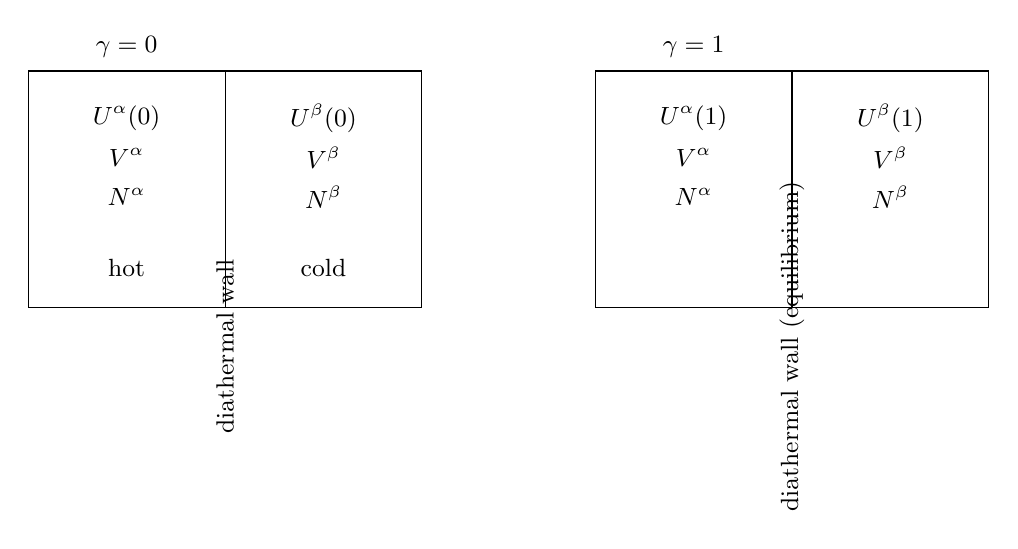
\begin{tikzpicture}[font=\small]
    % Left diagram: gamma = 0
    \draw (0,0) rectangle (5,3);
    \draw (2.5,0) -- (2.5,3);
    \node at (1.25,3.3) {$\gamma=0$};
    \node at (1.25,2.4) {$U^{\alpha}(0)$};
    \node at (1.25,1.9) {$V^{\alpha}$};
    \node at (1.25,1.4) {$N^{\alpha}$};
    \node at (1.25,0.5) {hot};
    \node at (3.75,2.4) {$U^{\beta}(0)$};
    \node at (3.75,1.9) {$V^{\beta}$};
    \node at (3.75,1.4) {$N^{\beta}$};
    \node at (3.75,0.5) {cold};
    \node[rotate=90] at (2.5,-0.5) {diathermal wall};

    % Right diagram: gamma = 1
    \begin{scope}[xshift=7.2cm]
        \draw (0,0) rectangle (5,3);
        \draw (2.5,0) -- (2.5,3);
        \node at (1.25,3.3) {$\gamma=1$};
        \node at (1.25,2.4) {$U^{\alpha}(1)$};
        \node at (1.25,1.9) {$V^{\alpha}$};
        \node at (1.25,1.4) {$N^{\alpha}$};
        \node at (3.75,2.4) {$U^{\beta}(1)$};
        \node at (3.75,1.9) {$V^{\beta}$};
        \node at (3.75,1.4) {$N^{\beta}$};
        \node[rotate=90] at (2.5,-0.5) {diathermal wall (equilibrium)};
    \end{scope}
\end{tikzpicture}
\end{document}
